% 1D Dirichlet sine decay -- case_1d.py (energy-coupled, EOS temperature).
% The sine profile is imposed through the DENSITY at uniform pressure,
%   rho(x) = rho0 Twall / (Twall + A sin(pi x/L)),   p = p0 = const.
% T is then recovered from the stiffened-gas EOS; weak compressible acoustics
% make u != 0 and set a small physics-driven error floor.
%
% Compile:  pdflatex setup_1d_energy.tex
\documentclass[border=6pt]{standalone}
\usepackage{amsmath}
\usepackage{tikz}
\usepackage{pgfplots}
\pgfplotsset{compat=1.18}
\usetikzlibrary{arrows.meta}

\definecolor{coldc}{RGB}{46,86,149}
\definecolor{hotc}{RGB}{171,57,52}
\definecolor{inkc}{RGB}{30,30,30}
\definecolor{rhoc}{RGB}{109,72,140}

\begin{document}
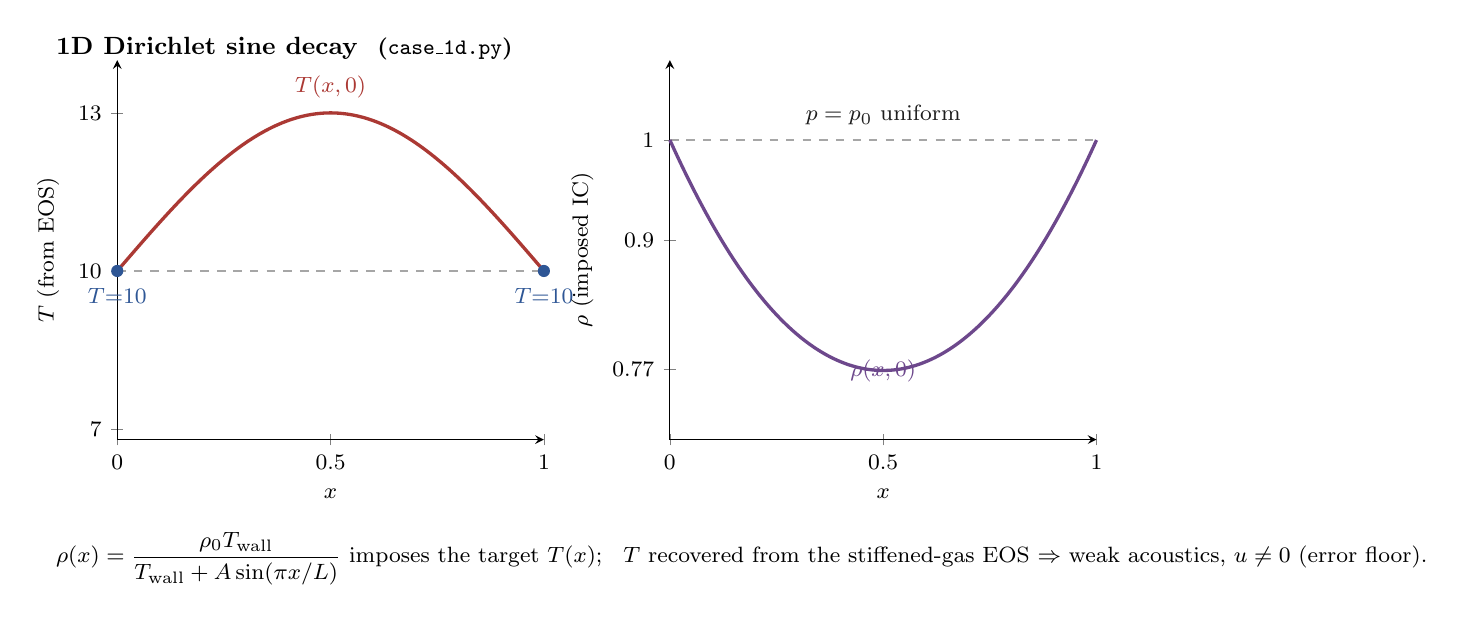
\begin{tikzpicture}[>=Stealth, font=\footnotesize]
% LEFT panel: recovered temperature T(x)
\begin{axis}[
  name=tax, width=7.0cm, height=6.4cm,
  xlabel={$x$}, ylabel={$T$ (from EOS)},
  xmin=0, xmax=1, ymin=6.8, ymax=14, axis lines=left, samples=160,
  xtick={0,0.5,1}, ytick={7,10,13}, enlargelimits=false, clip=false,
]
  \addplot[gray!70, dashed, thick, domain=0:1] {10};
  \addplot[hotc, very thick, domain=0:1] {10 + 3*sin(deg(pi*x))};
  \node[hotc, anchor=south] at (axis cs:0.5,13.1) {$T(x,0)$};
  \fill[coldc] (axis cs:0,10) circle (2.2pt);
  \fill[coldc] (axis cs:1,10) circle (2.2pt);
  \node[coldc, anchor=north, align=center] at (axis cs:0,9.85) {$T{=}10$};
  \node[coldc, anchor=north, align=center] at (axis cs:1,9.85) {$T{=}10$};
\end{axis}

% RIGHT panel: imposed density rho(x) (inverse of T at uniform pressure)
\begin{axis}[
  name=rax, at={(tax.east)}, anchor=west, xshift=1.6cm,
  width=7.0cm, height=6.4cm,
  xlabel={$x$}, ylabel={$\rho$ (imposed IC)},
  xmin=0, xmax=1, ymin=0.7, ymax=1.08, axis lines=left, samples=160,
  xtick={0,0.5,1}, ytick={0.77,0.9,1.0}, enlargelimits=false, clip=false,
]
  \addplot[gray!70, dashed, thick, domain=0:1] {1.0};
  % rho0 = 1, Twall = 10, A = 3  ->  10/(10 + 3 sin)
  \addplot[rhoc, very thick, domain=0:1] {10/(10 + 3*sin(deg(pi*x)))};
  \node[rhoc, anchor=north] at (axis cs:0.5,0.79) {$\rho(x,0)$};
  \node[inkc, anchor=south] at (axis cs:0.5,1.005) {$p=p_0$ uniform};
\end{axis}

\node[font=\bfseries\small, anchor=south west] at (-0.9,4.7)
  {1D Dirichlet sine decay \ \footnotesize(\texttt{case\_1d.py})};
\node[anchor=north west, align=left, font=\footnotesize] at (-0.9,-1.05)
  {$\rho(x)=\dfrac{\rho_0 T_{\text{wall}}}{T_{\text{wall}}+A\sin(\pi x/L)}$ imposes the target $T(x)$;\;\;
   $T$ recovered from the stiffened-gas EOS $\Rightarrow$ weak acoustics, $u\neq 0$ (error floor).};
\end{tikzpicture}
\end{document}
